\subsection*{Question 3.4}
The plot of the SVD.samples, can be seen in figure \ref{fig:q34}, then the y axe is the difference gene, and the x axe is the distance between the difference groups. The longer out the gene is joint, the more distance there are between the gene. This representation, is are good wait to group find together, sine we can set are max distance. and set are lien at that distance, an just fine all the grouping that are to the left of the line. This also mean, that we can set are number of grouping, and find the distance the gene need to have to get the number of grouping
\begin{figure}[!htbp]
  \centering
  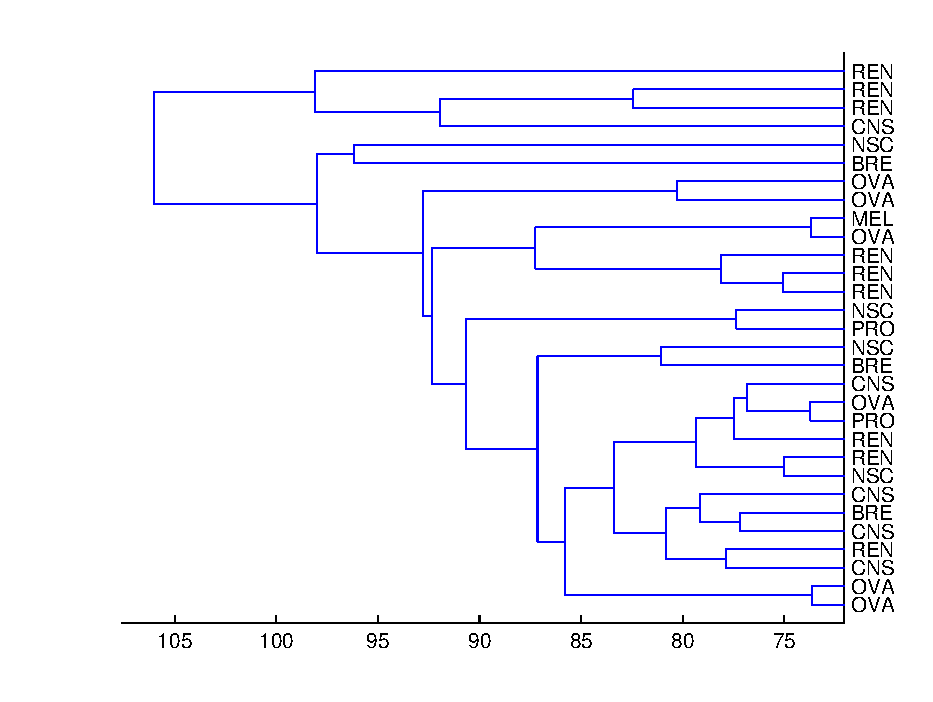
\includegraphics[width=0.85\textwidth]{./images/q34}
  \caption{Shows are plot over the SVD sample of difference gene.}
  \label{fig:q34}
\end{figure}

